% Options for packages loaded elsewhere
\PassOptionsToPackage{unicode}{hyperref}
\PassOptionsToPackage{hyphens}{url}
%
\documentclass[
  12 pt,
  a4paper,
]{article}
\usepackage{amsmath,amssymb}
\usepackage{setspace}
\usepackage{iftex}
\ifPDFTeX
  \usepackage[T1]{fontenc}
  \usepackage[utf8]{inputenc}
  \usepackage{textcomp} % provide euro and other symbols
\else % if luatex or xetex
  \usepackage{unicode-math} % this also loads fontspec
  \defaultfontfeatures{Scale=MatchLowercase}
  \defaultfontfeatures[\rmfamily]{Ligatures=TeX,Scale=1}
\fi
\usepackage{lmodern}
\ifPDFTeX\else
  % xetex/luatex font selection
  \setmainfont[]{Times New Roman}
\fi
% Use upquote if available, for straight quotes in verbatim environments
\IfFileExists{upquote.sty}{\usepackage{upquote}}{}
\IfFileExists{microtype.sty}{% use microtype if available
  \usepackage[]{microtype}
  \UseMicrotypeSet[protrusion]{basicmath} % disable protrusion for tt fonts
}{}
\makeatletter
\@ifundefined{KOMAClassName}{% if non-KOMA class
  \IfFileExists{parskip.sty}{%
    \usepackage{parskip}
  }{% else
    \setlength{\parindent}{0pt}
    \setlength{\parskip}{6pt plus 2pt minus 1pt}}
}{% if KOMA class
  \KOMAoptions{parskip=half}}
\makeatother
\usepackage{xcolor}
\usepackage[margin=1in]{geometry}
\usepackage{longtable,booktabs,array}
\usepackage{calc} % for calculating minipage widths
% Correct order of tables after \paragraph or \subparagraph
\usepackage{etoolbox}
\makeatletter
\patchcmd\longtable{\par}{\if@noskipsec\mbox{}\fi\par}{}{}
\makeatother
% Allow footnotes in longtable head/foot
\IfFileExists{footnotehyper.sty}{\usepackage{footnotehyper}}{\usepackage{footnote}}
\makesavenoteenv{longtable}
\usepackage{graphicx}
\makeatletter
\def\maxwidth{\ifdim\Gin@nat@width>\linewidth\linewidth\else\Gin@nat@width\fi}
\def\maxheight{\ifdim\Gin@nat@height>\textheight\textheight\else\Gin@nat@height\fi}
\makeatother
% Scale images if necessary, so that they will not overflow the page
% margins by default, and it is still possible to overwrite the defaults
% using explicit options in \includegraphics[width, height, ...]{}
\setkeys{Gin}{width=\maxwidth,height=\maxheight,keepaspectratio}
% Set default figure placement to htbp
\makeatletter
\def\fps@figure{htbp}
\makeatother
\setlength{\emergencystretch}{3em} % prevent overfull lines
\providecommand{\tightlist}{%
  \setlength{\itemsep}{0pt}\setlength{\parskip}{0pt}}
\setcounter{secnumdepth}{-\maxdimen} % remove section numbering
\ifLuaTeX
\usepackage[bidi=basic]{babel}
\else
\usepackage[bidi=default]{babel}
\fi
\babelprovide[main,import]{spanish}
\ifPDFTeX
\else
\babelfont{rm}[]{Times New Roman}
\fi
% get rid of language-specific shorthands (see #6817):
\let\LanguageShortHands\languageshorthands
\def\languageshorthands#1{}
\ifLuaTeX
  \usepackage{selnolig}  % disable illegal ligatures
\fi
\usepackage{bookmark}
\IfFileExists{xurl.sty}{\usepackage{xurl}}{} % add URL line breaks if available
\urlstyle{same}
\hypersetup{
  pdfauthor={Tomàs Ferrandis Moscardó},
  pdflang={es-ES},
  hidelinks,
  pdfcreator={LaTeX via pandoc}}

\title{U2: FERRAMENTES DE VIRTUALITZACIÓ}
\usepackage{etoolbox}
\makeatletter
\providecommand{\subtitle}[1]{% add subtitle to \maketitle
  \apptocmd{\@title}{\par {\large #1 \par}}{}{}
}
\makeatother
\subtitle{Aproximació al VirtualBox (instal·lació mínima)}
\author{Tomàs Ferrandis Moscardó}
\date{}

\begin{document}
\maketitle

{
\setcounter{tocdepth}{2}
\tableofcontents
}
\setstretch{1.5}
\newpage
\renewcommand\tablename{Tabla}

\begin{center}\rule{0.5\linewidth}{0.5pt}\end{center}

\section{1. Introducció}\label{introducciuxf3}

La virtualització és una tecnologia informàtica que permet crear entorns
virtuals dins de sistemes físics. En el nostre módul creraem Màquines
Virtuals.

En aquesta unitat farem una aproximació mitjançant l'eina gratuïta (i
sense suport!) d'Oracle \textbf{VM VirtualBox} amb la Llicència d'ús
gratuït (Personal Use License) que esn permet l'ús gratuït personal mai
comercial.

\subsection{1.1 Avantatges}\label{avantatges}

\begin{itemize}
\tightlist
\item
  \textbf{Reducció de costos}: Menys maquinari físic.
\item
  \textbf{Flexibilitat i escalabilitat}: Facilita la creació de nous
  entorns de proves o producció.
\item
  \textbf{Recuperació ràpida}: Facilita la recuperació davant de
  fallades.
\item
  \textbf{Espais de proves (aïllament)}: Ideal amb finalitat educativa o
  experimental.
\item
  \textbf{Eficiència en la utilització dels recursos:} Permet a diversos
  sistemes operatius funcionar simultàniament sobre el mateix maquinari.
\end{itemize}

\section{2. Màquines virtuals}\label{muxe0quines-virtuals}

\subsection{2.1 Definició}\label{definiciuxf3}

Una màquina virtual (MV) és una emulació d'ordinador independent dins
d'un ordinador físic mitjançant un software de sistema.

\subsection{2.2 Caracterísitiques:}\label{caracteruxedsitiques}

\begin{itemize}
\tightlist
\item
  Pot instal·lar-se un SO distint al de la màquina amfitriona.
\item
  Usa part dels recursos HW ( CPU, RAM, Discos\ldots).
\item
  Podem tindre'n més d'una en marxa en el mateix PC.
\item
  Podem comunicar-se per una xarxa virtual (interna) o no.
\item
  Poden accedir a carpetes del PC amfitrió.
\item
  Poden tenir accès a internet o no.
\item
  Poden exportar-se o executar-se en un disc extraïble en diferents PC
  ambfitrions.
\item
  Podem afegir HW vitrual facilment.
\item
  Podem instal·lar aplicacions.
\end{itemize}

\section{3 Tipus de virtualització}\label{tipus-de-virtualitzaciuxf3}

Centrant-nos en l'objectiu de mòdul de SOM, parlarem de la
\textbf{virtualizació de MV en local}. Així tindrem dos tipus basat en
dos tipus de \textbf{hipervisors}

\subsection{3.1 Hipervisors}\label{hipervisors}

És el software que permet l'execució de Máquinas Virtuales (VM).

\begin{itemize}
\item
  El SO principal sobre el que hem instal·lat l'hipervisor és el sistema
  operatiu amfitrió.
\item
  Els SOs de les MV són els SO invitats (guest)
\end{itemize}

Els hipervisors poden ser de 2 tipus:

\begin{itemize}
\item
  \textbf{Tipus 1} Funcionan directamente sobre el hardware. Exemples:
  Promox VE, VMware: ESX / vSphere Hypervisor, Microsoft Hyper-V Server,
  Citrix XenServer, citrix Hypervisor Xen
\item
  \textbf{Tipus 2} Funcionen sobre el SO amfitrió. Exemples: VirtualBox,
  VMWare Workstations/Player, Microsoft Virtual PC, QEMU Virt-Manager
\end{itemize}

\begin{figure}
\centering
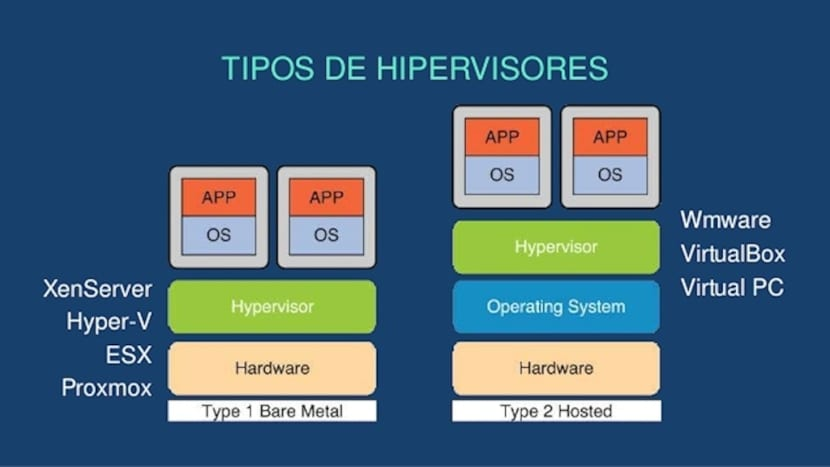
\includegraphics{png/tiposVirtualizadores.jpg}
\caption{\emph{Figura 1: Tipus de Hipervisors}}
\end{figure}

\subsection{3.2 Altres}\label{altres}

Hi ha més tipus de virutalització que podeu investigar però no és
objecte del mòdul de SOM.

\section{4. Oracle VM VirtualBox}\label{oracle-vm-virtualbox}

\subsection{\texorpdfstring{4.1 Instal·lació de VirtualBox \emph{Ho heu
de fer a
casa}}{4.1 Instal·lació de VirtualBox Ho heu de fer a casa}}\label{installaciuxf3-de-virtualbox-ho-heu-de-fer-a-casa}

\begin{itemize}
\tightlist
\item
  \textbf{Requisits del sistema:} Verificar les especificacions mínimes
  del sistema per a la instal·lació.
\item
  \textbf{Procés d'instal·lació:} Descarregar l'instal·lador des del
  lloc web oficial de VirtualBox. Seguir les instruccions per
  instal·lar-lo en els diferents sistemes operatius com Windows , Linux
  i macOS.
\end{itemize}

\href{}{Video Tutorial Windows 1x}

\href{}{Video Tutorial Linux}

\subsection{4.2 Entorn i barres dels
VirtualBox}\label{entorn-i-barres-dels-virtualbox}

\emph{Apartat poc important: 4.2}

\textbf{Entorn:}

\begin{itemize}
\tightlist
\item
  \textbf{Interfície d'usuari:} La interfície inclou la llista de
  màquines virtuals, opcions de configuració, i els logs de sistema.
\item
  \textbf{Seccions principals:} L'espai de treball principal on es poden
  veure i gestionar les màquines virtuals existents.
\end{itemize}

\textbf{Barra de ferramentes:}

\begin{itemize}
\tightlist
\item
  \textbf{Funcions principals:} La barra de ferramentes proporciona
  accés ràpid a funcions com iniciar, aturar, i suspendre màquines
  virtuals.
\item
  \textbf{Accions ràpides:} Permet realitzar accions com clonar, crear
  instantànies i accedir a la configuració ràpida de les màquines
  virtuals.
\end{itemize}

\textbf{Barra de menús:}

\begin{itemize}
\tightlist
\item
  \textbf{Gestió de discos virtuals:} Crear, eliminar i modificar discos
  virtuals associats a les màquines virtuals.
\item
  \textbf{Imatges ISO:} Afegir i gestionar imatges ISO utilitzades per
  instal·lar sistemes operatius o aplicacions.
\end{itemize}

\subsection{4.3 Importació i
exportació}\label{importaciuxf3-i-exportaciuxf3}

\begin{itemize}
\tightlist
\item
  \textbf{Importació:} Procediment per importar màquines virtuals des de
  formats com OVF o \textbf{OVA}
\item
  \textbf{Exportació:} Procediment per exportar màquines virtuals per a
  compartir o crear còpies de seguretat.
\end{itemize}

\begin{quote}
Nota:

Són procediments lents. Una opció més viable és crear la MV en un disc
extraible si el teu PC té un bon port USB 3.
\end{quote}

\subsection{4.4 Administració de medis
virtuals}\label{administraciuxf3-de-medis-virtuals}

\subsubsection{4.4.1 La Unitat de
magatzenament}\label{la-unitat-de-magatzenament}

Podem indicar on estan les ISO. - del SO a instal·lar - del
GuestAdditions ( ho vorem) - altre software (MS Office, per exemple)

En l'apartat de Sistema indiquem el que emularia al \textbf{Boot oder}
de la BIOS/UEFI. I ens assegurem que la MV inicie a partir del DVD.

\subsubsection{4.4.2 Discos}\label{discos}

En \textbf{VirtualBox}, quan crees un disc dur virtual, tens tres
possibles formats de fitxers.

\begin{enumerate}
\def\labelenumi{\arabic{enumi}.}
\tightlist
\item
  \textbf{VDI (VirtualBox Disk Image)}:

  \begin{itemize}
  \tightlist
  \item
    Aquest és el format \textbf{natiu de VirtualBox}.
  \item
    Ofereix compatibilitat completa amb totes les funcionalitats de
    VirtualBox, com la \textbf{mida dinàmica o fixa}.
  \item
    És ideal si només utilitzaràs el disc amb VirtualBox com serà el
    nostre cas.
  \end{itemize}
\item
  \textbf{VHD (Virtual Hard Disk)}:

  \begin{itemize}
  \tightlist
  \item
    Aquest és un format utilitzat principalment per Microsoft i
    aplicacions com Hyper-V (el virtualitzador integrat en Windows)
  \item
    És útil si necessites compartir el disc dur virtual amb sistemes
    Microsoft o altres aplicacions de virtualització que suporten aquest
    format.
  \end{itemize}
\item
  \textbf{VMDK (Virtual Machine Disk)}:

  \begin{itemize}
  \tightlist
  \item
    Aquest format és utilitzat per VMware, un altre software de
    virtualització.
  \item
    És adequat si necessites moure màquines virtuals entre VirtualBox i
    VMware.
  \end{itemize}
\end{enumerate}

\textbf{VDI} és el més eficient si només utilitzes \textbf{VirtualBox} i
serà el que usarem.

\begin{figure}
\centering
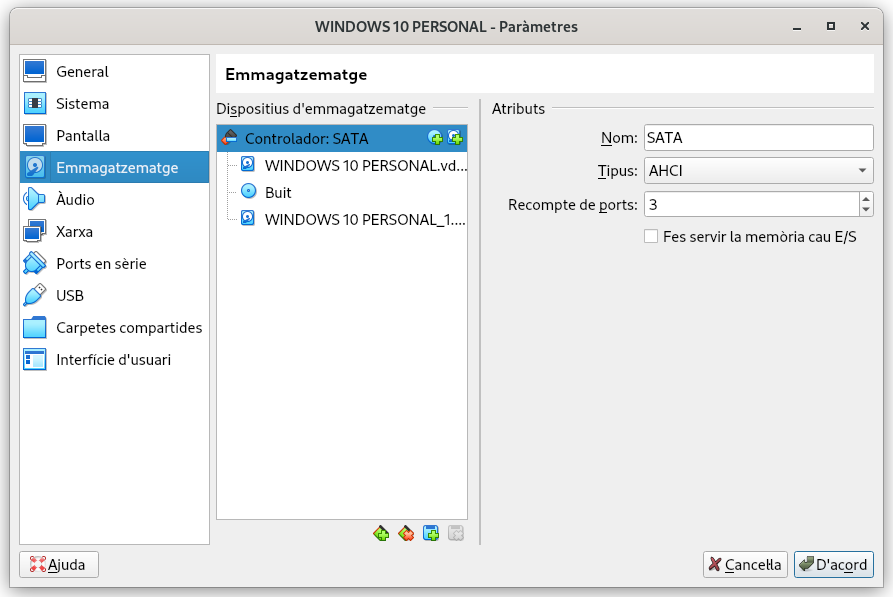
\includegraphics{png/4Emmagatzematge.png}
\caption{\emph{Figura 2:Emmagatzematge}}
\end{figure}

\subsubsection{4.4.3 Boot Order}\label{boot-order}

El \textbf{``boot order''} (ordre d'arrencada) es la seqüència en què el
sistema (la UEFI o BIO) busca dispositius per arrencar un sistema
operatiu quan l'ordinador es reinicia per carregar un sistema operatiu.

\begin{itemize}
\tightlist
\item
  \textbf{Disquetera} (OBSOLET.Desactivar).
\item
  \textbf{Unitats USB} (memòries USB, dispositius externs. NO operativa
  en VirtualBox).
\item
  \textbf{Unitats CD/DVD} (lectors de CD o DVD. La que usarem en
  VirtualBox).
\item
  \textbf{Disc dur o SSD} (on normalment està instal·lat el sistema
  operatiu).
\item
  \textbf{Xarxa} (per arrencar des d'un servidor en una xarxa,
  utilitzant tècniques com PXE).
\end{itemize}

La configuració del boot order es fa a través de la configuració del
BIOS o UEFI del sistema. Accedeixes a aquesta configuració generalment
prem el teclat \texttt{F2}, \texttt{Delete}, \texttt{Esc}

\subsubsection{Usos}\label{usos}

\begin{itemize}
\tightlist
\item
  \textbf{Instal·lació de Sistemes Operatius:} Per instal·lar el SO des
  de xarxa, USB o CD/DVD.
\item
  \textbf{Resolució de Problemes:} Si el sistema no arrenca
  correctament, pot ser útil modificar el boot order per intentar
  arrencar des d'un dispositiu de recuperació o un live CD.
\end{itemize}

\subsection{4.5 Configuració d'una màquina
virtual}\label{configuraciuxf3-duna-muxe0quina-virtual}

\subsubsection{Pantalla}\label{pantalla}

Pot ser la configuració ens done problemes, la canviem ací:

\begin{figure}
\centering
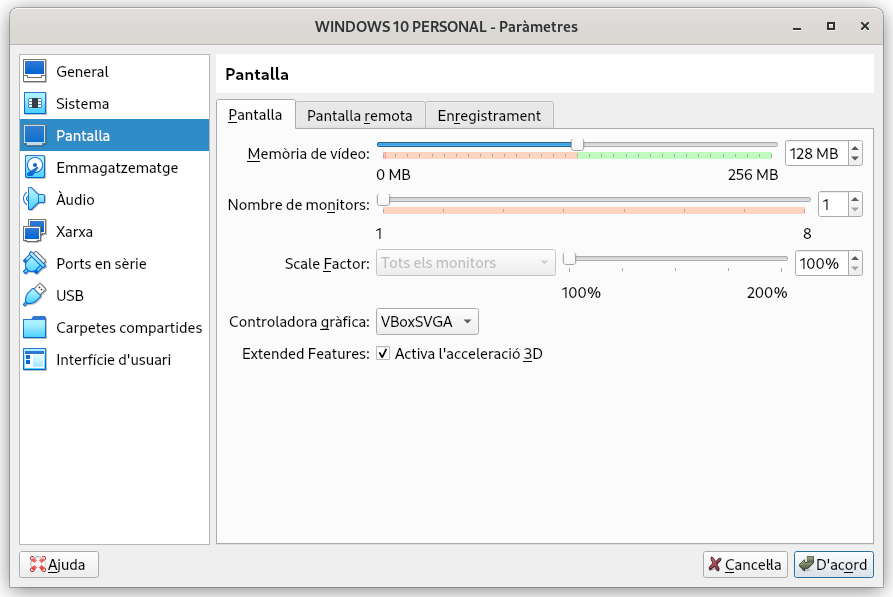
\includegraphics{png/3Pantalla.png}
\caption{\emph{Figura 3: Pantalla}}
\end{figure}

\subsubsection{USB}\label{usb}

L'accés a USB no sol anar massa bé en VirtualBox i pot donar algun
problema segons el SO que instal·lem. 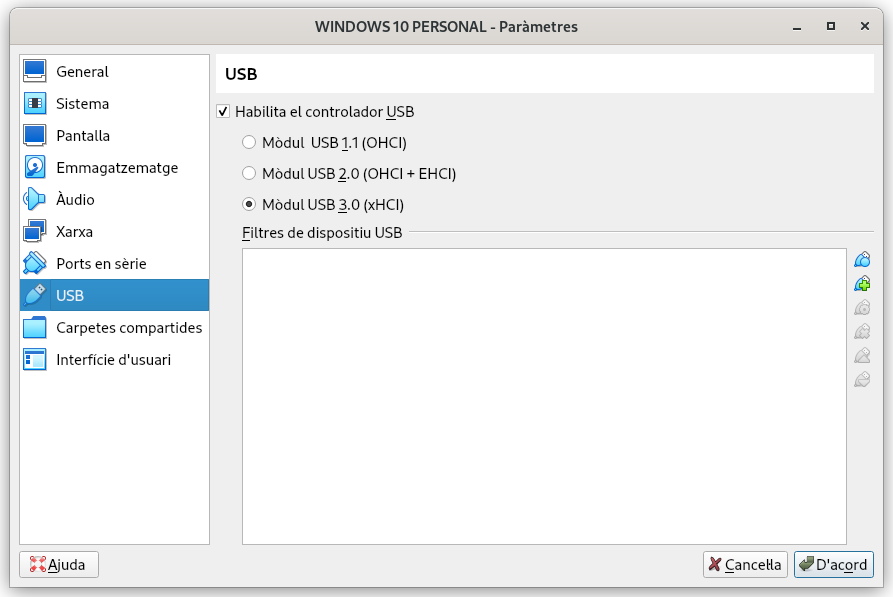
\includegraphics{png/8USB.png}

\subsubsection{4.5.1 Sistema}\label{sistema}

\begin{figure}
\centering
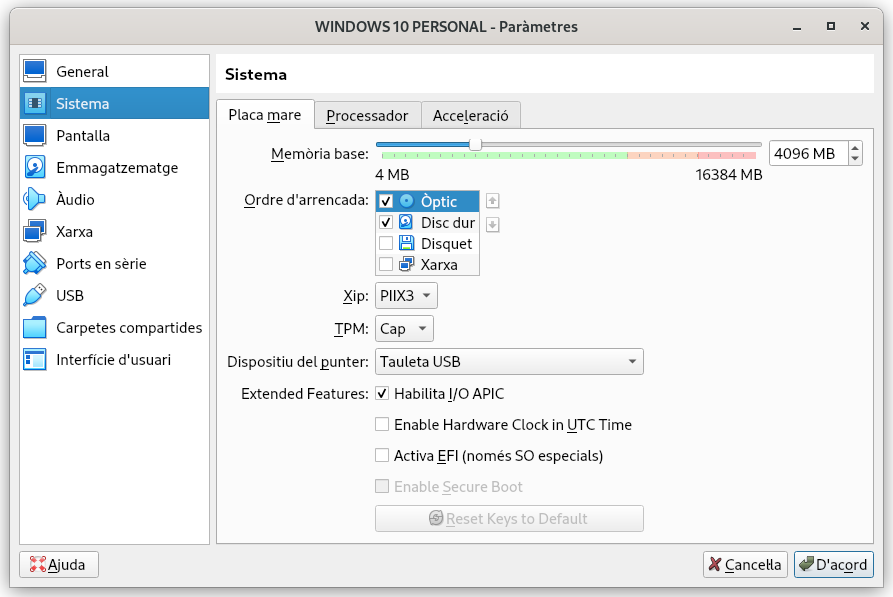
\includegraphics{png/2Sistema.png}
\caption{\emph{Figura 5:Sistema}}
\end{figure}

\begin{enumerate}
\def\labelenumi{\arabic{enumi}.}
\tightlist
\item
  \textbf{Xip (Processador Virtual)}:

  \begin{itemize}
  \tightlist
  \item
    \textbf{Funció}: Configura el tipus i la quantitat de processadors
    virtuals que utilitza la màquina virtual.
  \end{itemize}
\item
  \textbf{TPM (Trusted Platform Module)}:

  \begin{itemize}
  \tightlist
  \item
    \textbf{Funció}: Proporciona seguretat criptogràfica a nivell de
    maquinari per emmagatzemar claus i dades sensibles.
  \end{itemize}
\item
  \textbf{Habilita I/O APIC}:

  \begin{itemize}
  \tightlist
  \item
    \textbf{Funció}: Millora la gestió d'interrupcions, especialment en
    sistemes amb múltiples processadors o nuclis.
  \end{itemize}
\item
  \textbf{Activa EFI (Extensible Firmware Interface)}:

  \begin{itemize}
  \tightlist
  \item
    \textbf{Funció}: Substitueix el BIOS tradicional amb una interfície
    de firmware moderna que suporta arrencada des de discs GPT i altres
    funcions avançades.
  \end{itemize}
\end{enumerate}

\emph{Taula 1: Resum de les opcions de configuració de la màquina
virtual per SO.}

\begin{longtable}[]{@{}
  >{\raggedright\arraybackslash}p{(\columnwidth - 6\tabcolsep) * \real{0.1463}}
  >{\raggedright\arraybackslash}p{(\columnwidth - 6\tabcolsep) * \real{0.2744}}
  >{\raggedright\arraybackslash}p{(\columnwidth - 6\tabcolsep) * \real{0.2683}}
  >{\raggedright\arraybackslash}p{(\columnwidth - 6\tabcolsep) * \real{0.3110}}@{}}
\toprule\noalign{}
\begin{minipage}[b]{\linewidth}\raggedright
\textbf{Opció}
\end{minipage} & \begin{minipage}[b]{\linewidth}\raggedright
\textbf{Ubuntu}
\end{minipage} & \begin{minipage}[b]{\linewidth}\raggedright
\textbf{Windows 10}
\end{minipage} & \begin{minipage}[b]{\linewidth}\raggedright
\textbf{Windows 11}
\end{minipage} \\
\midrule\noalign{}
\endhead
\bottomrule\noalign{}
\endlastfoot
\textbf{Xip (Processador Virtual)} & Configuració per defecte és
suficient & Configuració per defecte és suficient & Configuració per
defecte, amb almenys 2 nuclis \\
\textbf{TPM (Trusted Platform Module)} & No necessari & No necessari &
Necessari; utilitza solucions alternatives per simular TPM \\
\textbf{Habilita I/O APIC} & Recomanat per a millor rendiment &
Recomanat per a millor rendiment & Recomanat per a millor rendiment \\
\textbf{Activa EFI} & Opcional, segons el disc (GPT o MBR) & Recomanat
si utilitzes un disc GPT & Necessari; el disc ha de ser GPT \\
\end{longtable}

\subsubsection{4.5.2 Xarxa}\label{xarxa}

\begin{figure}
\centering
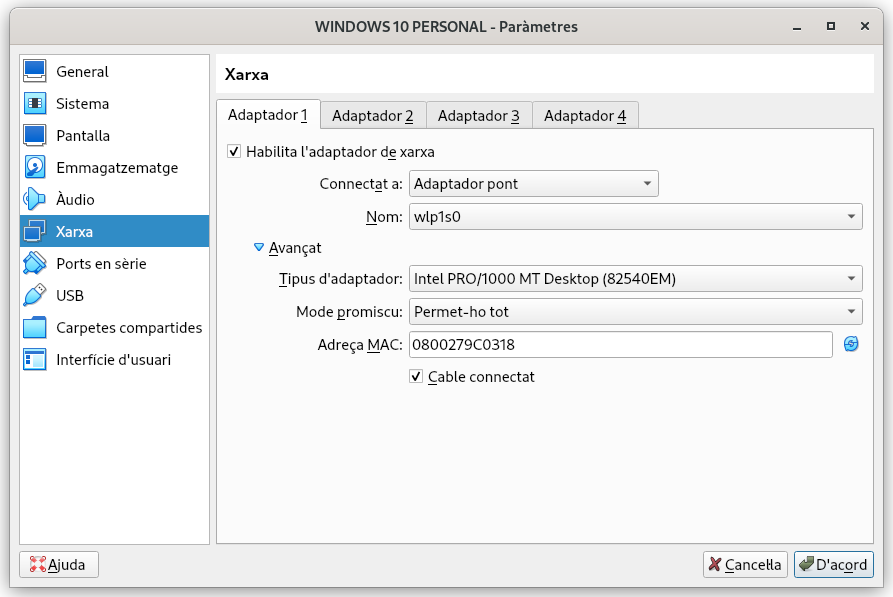
\includegraphics{png/6Adaptador.png}
\caption{\emph{Figura 6: Adaptador (de xarxa)}}
\end{figure}

En aquest punt convé detindre'ns en l'apartat de la configuració de
xarxa per dos raons:

\begin{itemize}
\item
  Podem fer comporvacions de les IPs que tindrà la màquina segons la
  configuració que fem ara al ``HW virtual''. Qüestió relacionada amb el
  mòdul de XAL.
\item
  Per al curs de 2n ho usarem més en els mòduls de SOX i SEX.
\end{itemize}

De totes les opcions que ens apareixen anem a centrar-nos en les que més
ens interessen.

\begin{itemize}
\item
  \textbf{Adaptador pont} fa que la MV aparega com un PC més de la xarxa
  local real de l'aula o de ta casa. Tindrà una IP del mateix rang que
  la de l'amfitrió si ha sigut porporcionada pel servei del router.
\item
  \textbf{NAT} Assigan una IP de rang (inclús de classe) ditinta a la
  del teu PC amfitrió.
\item
  \textbf{XARXA INTERNA} A l'igual que l'anterior però ens permet
  assignar un \textbf{nom a la xarxa}.
\end{itemize}

\emph{Taula 2: Resum característiques xarxa VirtualBox}

\begin{longtable}[]{@{}
  >{\raggedright\arraybackslash}p{(\columnwidth - 8\tabcolsep) * \real{0.2000}}
  >{\raggedright\arraybackslash}p{(\columnwidth - 8\tabcolsep) * \real{0.2000}}
  >{\raggedright\arraybackslash}p{(\columnwidth - 8\tabcolsep) * \real{0.2000}}
  >{\raggedright\arraybackslash}p{(\columnwidth - 8\tabcolsep) * \real{0.2000}}
  >{\raggedright\arraybackslash}p{(\columnwidth - 8\tabcolsep) * \real{0.2000}}@{}}
\toprule\noalign{}
\begin{minipage}[b]{\linewidth}\raggedright
Té accés a internet
\end{minipage} & \begin{minipage}[b]{\linewidth}\raggedright
Pot comunicar-se amb altres MV
\end{minipage} & \begin{minipage}[b]{\linewidth}\raggedright
Es pot comunicar amb la màquina real
\end{minipage} & \begin{minipage}[b]{\linewidth}\raggedright
Hem de configurar alguna cosa a Linux/Windows
\end{minipage} & \begin{minipage}[b]{\linewidth}\raggedright
\end{minipage} \\
\midrule\noalign{}
\endhead
\bottomrule\noalign{}
\endlastfoot
NAT & Sí & No & No & No \\
XARXA INTERNA & No & Sí & No & Sí \\
PONT (BRIDGE) & Sí & Sí & Sí & No \\
\end{longtable}

\subsection{4.6 Ús de carpetes
compartides}\label{uxfas-de-carpetes-compartides}

\begin{figure}
\centering
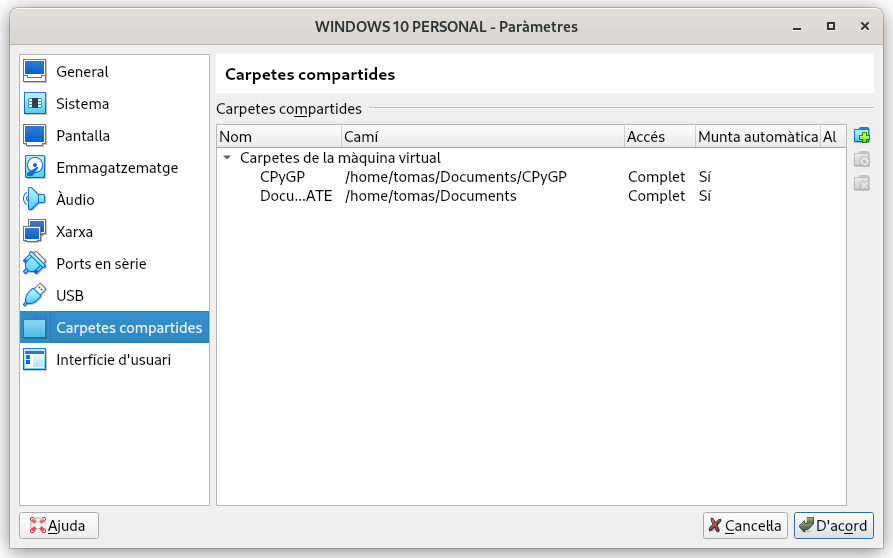
\includegraphics{png/9CarpetesCompartides.png}
\caption{\emph{Figura 7: Carpetes compartides}}
\end{figure}

\begin{itemize}
\tightlist
\item
  \textbf{Configuració:} Configurar carpetes compartides entre el
  sistema host (amfritrió) i les màquines virtuals per facilitar
  l'intercanvi de fitxers.
\item
  \textbf{Gestió de permisos:} Assegurar que les carpetes compartides
  tenen els permisos adequats per accedir i modificar els fitxers des de
  les màquines virtuals.
\end{itemize}

Exemples pràctics habituals d'ús de les carpetes compartides:

\begin{enumerate}
\def\labelenumi{\arabic{enumi}.}
\item
  Usar programes de Linux i Windows sobre els mateixos fitxers. Exmeple:
  El meu portatil té un Ubuntu i, a vegades vull usar el MS Office. Tinc
  una màquina virutal amb Windows 11 amb el MS Office des d'on accedisc
  a la carpeta \emph{/home/tomas/Documents}
\item
  Estem treballant a classe o casa en la MV Lubuntu i fem captures de
  pantalla, documents etc\ldots{} des de la MV per no anar alternant
  d'entorn (tampoc té massa compliació), podem guardar directament a la
  carpeta compartida des de la MV.
\end{enumerate}

\section{5. Alternatives de
virtualització}\label{alternatives-de-virtualitzaciuxf3}

\subsection{5.1 VMware}\label{vmware}

\begin{itemize}
\tightlist
\item
  \textbf{VMware Workstation:} Aplicació de virtualització de maquinari
  per a usuaris de PC i servidors, amb funcionalitats avançades per a
  entorns de desenvolupament i proves.
\item
  \textbf{VMware Player:} Versió gratuïta per executar màquines
  virtuals, adequada per a usuaris individuals.
\end{itemize}

\subsection{5.2 Altres}\label{altres-1}

\begin{itemize}
\tightlist
\item
  \textbf{Parallels Desktop:} Solució de virtualització específica per a
  macOS, permet executar sistemes operatius Windows i altres sobre Macs.
\item
  \textbf{Hyper-V:} Tecnologia de virtualització de Microsoft integrada
  en Windows 10 i Windows Server, ofereix funcions avançades per a la
  creació i gestió de màquines virtuals.
\end{itemize}

(\emph{No cal estudiar a partir d'ací})

\begin{itemize}
\tightlist
\item
  \textbf{KVM (Kernel-based Virtual Machine):} Solució de virtualització
  per a Linux basada en el nucli, ofereix un entorn robust per a la
  creació i gestió de màquines virtuals.
\item
  \textbf{Xen:} Hypervisor de codi obert que permet la virtualització de
  maquinari per a diversos sistemes operatius i entorns de servidor.
\end{itemize}

\end{document}
